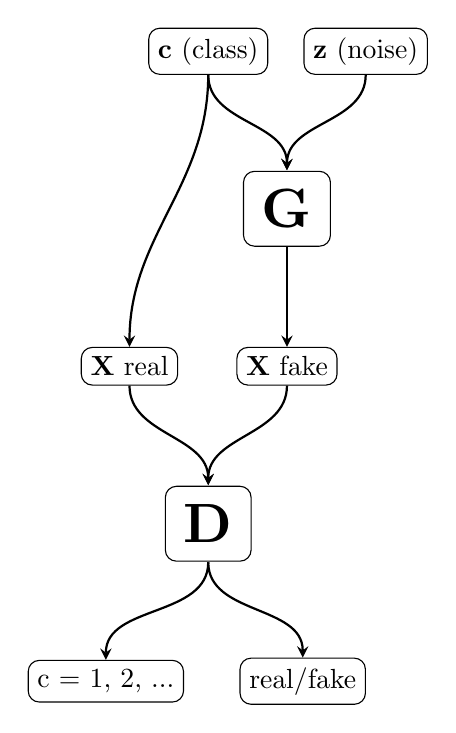
\begin{tikzpicture}[node distance=2cm]

\tikzstyle{zinput} = [rectangle, rounded corners, text centered, draw=black]%, fill=red!30]
\tikzstyle{generator} = [rectangle, rounded corners, text centered, draw=black]%, fill=red!30]
\tikzstyle{X real} = [rectangle, rounded corners, text centered, draw=black]%, fill=red!30]
\tikzstyle{X fake} = [rectangle, rounded corners, text centered, draw=black]%, fill=red!30]
\tikzstyle{X real} = [rectangle, rounded corners, text centered, draw=black]%, fill=red!30]
\tikzstyle{discriminator} = [rectangle, rounded corners, text centered, draw=black]%, fill=red!30]
\tikzstyle{real/fake} = [rectangle, rounded corners, text centered, draw=black]%, fill=red!30]
\tikzstyle{coutput} = [rectangle, rounded corners, text centered, draw=black]%, fill=red!30]

\tikzstyle{arrow} = [thick,->,>=stealth]

\node (r) [X real] {\textbf{X} real};
\node (f) [X fake, right of = r] {\textbf{X} fake};
\node (G) [generator,above of = f, scale = 2] {\textbf{G}};
\node (z) [zinput] [zinput, above of = G, xshift = 1cm] {\textbf{z} (noise)};
\node (c) [coutput, left of = z] {\textbf{c} (class)};
\node (D) [discriminator, below of = f, xshift = -1cm, scale = 2] {\textbf{D}};
\node (rf) [real/fake, below of = D, xshift = 1.2cm] {real/fake};
\node (co) [coutput, left of = rf, xshift = -0.5cm] {c = 1, 2, ...};

\draw [arrow] (z) edge[out=270,in=90] (G);
\draw [arrow] (c) edge[out=270,in=90] (G);
\draw [arrow] (c) edge[out=270,in=90] (r);
\draw [arrow] (G) -- (f);
\draw [arrow] (r) edge[out=270,in=90] (D);
\draw [arrow] (f) edge[out=270,in=90] (D);
\draw [arrow] (D) edge[out=270,in=90] (rf);
\draw [arrow] (D) edge[out=270,in=90] (co);

\end{tikzpicture}